% Copyright 2004 by Till Tantau <tantau@users.sourceforge.net>.
%
% In principle, this file can be redistributed and/or modified under
% the terms of the GNU Public License, version 2.
%
% However, this file is supposed to be a template to be modified
% for your own needs. For this reason, if you use this file as a
% template and not specifically distribute it as part of a another
% package/program, I grant the extra permission to freely copy and
% modify this file as you see fit and even to delete this copyright
% notice. 



\documentclass[xcolor={table,dvipsnames,usenames}]{beamer}
\usepackage{empheq}
\usepackage{color}
\definecolor{myblue}{rgb}{.8, .8, 1}
\newlength\mytemplen
\newsavebox\mytempbox

\makeatletter
\newcommand\mybluebox{%
	\@ifnextchar[%]
	{\@mybluebox}%
	{\@mybluebox[0pt]}}

\def\@mybluebox[#1]{%
	\@ifnextchar[%]
	{\@@mybluebox[#1]}%
	{\@@mybluebox[#1][0pt]}}

\def\@@mybluebox[#1][#2]#3{
	\sbox\mytempbox{#3}%
	\mytemplen\ht\mytempbox
	\advance\mytemplen #1\relax
	\ht\mytempbox\mytemplen
	\mytemplen\dp\mytempbox
	\advance\mytemplen #2\relax
	\dp\mytempbox\mytemplen
	\colorbox{myblue}{\hspace{1em}\usebox{\mytempbox}\hspace{1em}}}

\makeatother
%\usepackage[utf8]{hyperref}
%\hypersetup{
%	colorlinks=true,
%	linkcolor=blue,
%	filecolor=magenta,      
%	urlcolor=cyan,
%}
% There are many different themes available for Beamer. A comprehensive
% list with examples is given here:
% http://deic.uab.es/~iblanes/beamer_gallery/index_by_theme.html
% You can uncomment the themes below if you would like to use a different
% one:
%\usetheme{AnnArbor}
%\usetheme{Antibes}
%\usetheme{Bergen}
%\usetheme{Berkeley}
%\usetheme{Berlin}
%\usetheme{Boadilla}
%\usetheme{boxes}
%\usetheme{CambridgeUS}
%\usetheme{Copenhagen}
%\usetheme{Darmstadt}
%\usetheme{default}
%\usetheme{Frankfurt}
%\usetheme{Goettingen}
%\usetheme{Hannover}
%\usetheme{Ilmenau}
%\usetheme{JuanLesPins}
%\usetheme{Luebeck}
\usetheme{Madrid}
%\usetheme{Malmoe}
%\usetheme{Marburg}
%\usetheme{Montpellier}
%\usetheme{PaloAlto}
%\usetheme{Pittsburgh}
%\usetheme{Rochester}
%\usetheme{Singapore}
%\usetheme{Szeged}
%\usetheme{Warsaw}
%gets rid of bottom navigation bars
%\setbeamertemplate{footline}[frame number]{}

%gets rid of bottom navigation symbols
\setbeamertemplate{navigation symbols}{}
%\usepackage[dvipsnames]{xcolor}
%gets rid of footer
%will override 'frame number' instruction above
%comment out to revert to previous/default definitions
%\setbeamertemplate{footline}{}
\setbeamertemplate{footline}[page number]


\title{Hardness vs. Randomness}

% A subtitle is optional and this may be deleted
%\subtitle{Optional Subtitle}

\author{Rahul Gupta\inst{1}, 
	Shubham Sharma\inst{1}}
% - Give the names in the same order as the appear in the paper.
% - Use the \inst{?} command only if the authors have different
%   affiliation.

\institute[Universities of Somewhere and Elsewhere] % (optional, but mostly needed)
{
  \inst{1}%
  Indian Institute of Technology Kanpur, India}
% - Use the \inst command only if there are several affiliations.
% - Keep it simple, no one is interested in your street address.

\date{18 April 2019}
% - Either use conference name or its abbreviation.
% - Not really informative to the audience, more for people (including
%   yourself) who are reading the slides online

%\subject{Theoretical Computer Science}
% This is only inserted into the PDF information catalog. Can be left
% out. 

% If you have a file called "university-logo-filename.xxx", where xxx
% is a graphic format that can be processed by latex or pdflatex,
% resp., then you can add a logo as follows:

% \pgfdeclareimage[height=0.5cm]{university-logo}{university-logo-filename}
% \logo{\pgfuseimage{university-logo}}

% Delete this, if you do not want the table of contents to pop up at
% the beginning of each subsection:
%\AtBeginSubsection[]
%{
%  \begin{frame}<beamer>{Outline}
%    \tableofcontents[currentsection,currentsubsection]
%  \end{frame}
%}
\usepackage[font=scriptsize,skip=4pt]{caption}
\usepackage{multirow}
\usepackage{color, colortbl}
\definecolor{LightCyan}{rgb}{0.88,1,1}
\definecolor{darkblue}{rgb}{0.0,0.0,1}
\hypersetup{colorlinks,breaklinks,linkcolor=darkblue,urlcolor=darkblue,anchorcolor=darkblue,citecolor=darkblue}
% Let's get started
\begin{document}

\newcommand{\ddnnf}{\ensuremath{\mathsf{dag}}}
\newcommand{\Poly}{\ensuremath{\mathsf{P}}}
\newcommand{\NP}{\ensuremath{\mathsf{NP}}}
\newcommand{\WAPS}{\ensuremath{\mathsf{WAPS}}}
\newcommand{\KUS}{\ensuremath{\mathsf{KUS}}}
\newcommand{\DSPACE}{\ensuremath{\mathsf{DSPACE}}}
\newcommand{\EXPTIME}{\ensuremath{\mathsf{EXPTIME}}}
\newcommand{\RNC}{\ensuremath{\mathsf{RNC}}}
\newcommand{\BPP}{\ensuremath{\mathsf{BPP}}}
\newcommand{\DTIME}{\ensuremath{\mathsf{DTIME}}}
\newcommand{\RTIME}{\ensuremath{\mathsf{RTIME}}}
\newcommand{\WeightGen}{\ensuremath{\mathsf{WeightGen}}}
\newcommand{\prob}{\ensuremath{\mathsf{Pr}}}
\newcommand{\UniGen}{\ensuremath{\mathsf{UniGen2}}}
\newcommand{\satisfying}[1]{\ensuremath{R_{#1}}} %
\newcommand{\satisfyingv}[2]{\ensuremath{R_{#1\downarrow #2}}}
\newcommand{\Sampler}{\ensuremath{\mathsf{Sampler}}}
\newcommand{\sampleList}{\ensuremath{\mathsf{SampleList}}}
\newcommand{\Shuffle}{\ensuremath{\mathsf{Shuffle}}}
\newcommand{\Append}{\ensuremath{\mathsf{Append}}}
\newcommand{\Stitch}{\ensuremath{\mathsf{Stitch}}}
\newcommand{\IS}{\ensuremath{\mathsf{IS}}}
\newcommand{\normalize}{\ensuremath{\mathsf{Normalize}}}
\newcommand{\WCounter}{\ensuremath{\mathsf{WAnnotate}}}
\newcommand{\PCompile}{\ensuremath{\mathsf{PCompile}}}

\definecolor{ao(english)}{rgb}{0.0, 0.5, 0.0}

\begin{frame}
  \titlepage
  \begin{center}
  	\footnote{\href{https://www.math.ias.edu/avi/node/780}{https://www.math.ias.edu/avi/node/780}}
%  	The tool is available online \href{https://github.com/meelgroup/WAPS}{\textcolor{blue}{https://github.com/meelgroup/WAPS}}
  \end{center}
  
\end{frame}

\section{Pseudorandom Generator}
\begin{frame}{Pseudorandom Generator (PRG)}
\begin{itemize}
	\item $G: \{0,1\}^r \rightarrow \{0,1\}^n$ is a {\underline{pseudorandom generator}} such that it \textcolor{red}{appears random (fools)} to a \textcolor{blue}{class of test functions}.
	\pause
	\item $G~\epsilon$-fools $F$ if $\forall f \in F$ such that $f: \{0,1\}^n \rightarrow \{0,1\}$
	$$\Big|\prob\big[f(y)\big] -  \prob\big[f(G(x))\big]\Big| \leq \epsilon$$
	where $x$ is choosen uniformly from $\{0,1\}^r$ and $y$ from $\{0,1\}^n$
	\pause
	\begin{itemize}
		\item[--] Parity-function.
		\item[--] Polynomial-funtions.
		\item[--] \textcolor{blue}{Boolean-circuits}.
	\end{itemize}
	\pause
	\item G is a \textcolor{blue}{quick pseudorandom generator} if it runs in \underline{deterministic} time \textcolor{red}{exponential} in its input size, $G \in \DTIME (2^{O(r)})$.
	\begin{itemize}
		\item[--] \textcolor{blue}{quality of the output} -- $n,\epsilon$
		\item[--] \textcolor{blue}{price} -- $r$
	\end{itemize}
\end{itemize}
\end{frame}
\begin{frame}{Motivation}
\begin{itemize}
	\item If there exists a quick pseudorandom generator $G: \log(n) \rightarrow n$ then for any time constructible bound $t=t(n):$ $$\RTIME(t) \subset \DTIME(2^{O(\log(t^2))})$$
	\pause
	\begin{center}
			        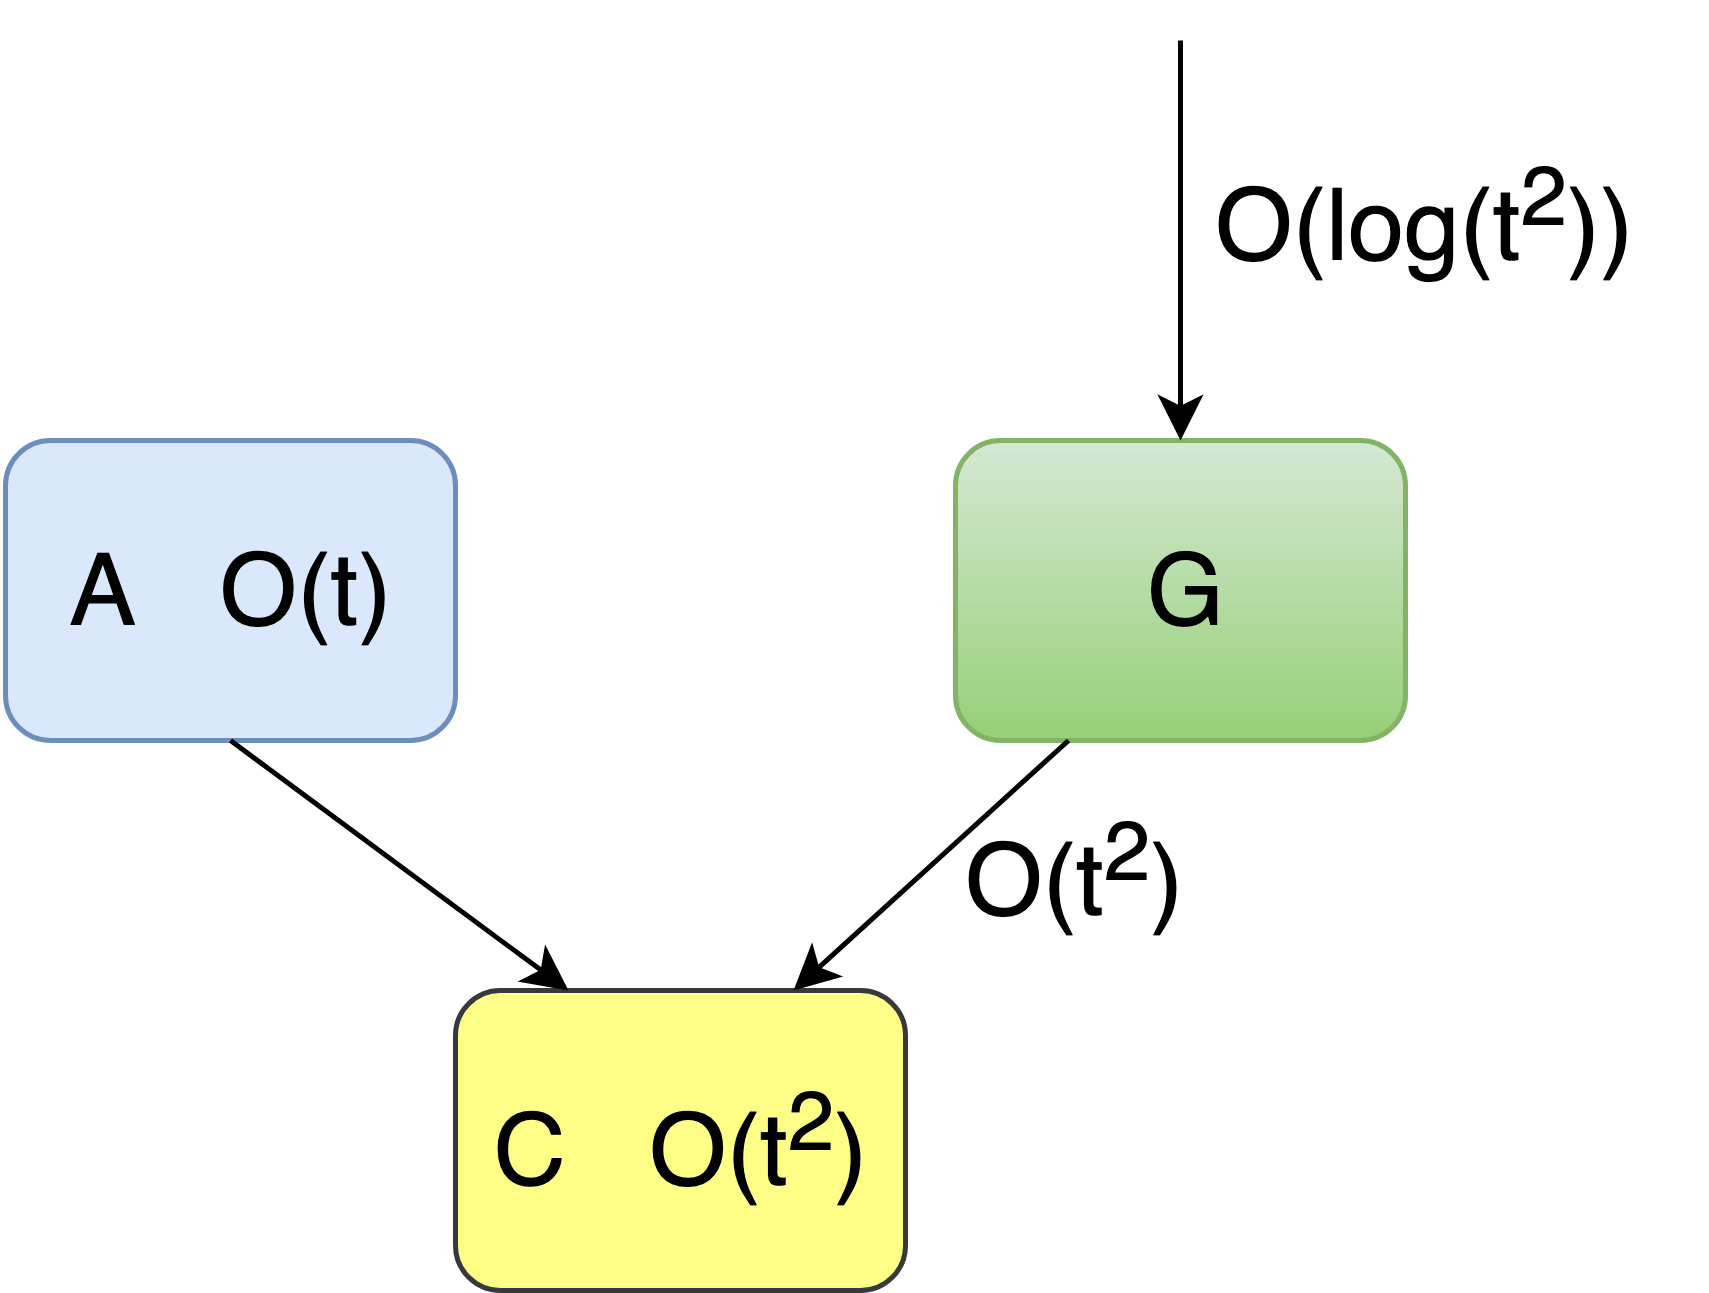
\includegraphics[width=0.4\columnwidth]{figures/RandomSimulation}
	\end{center}
\pause
\item  Simulate $A$ deterministically, by trying all the possible random seeds and taking a majority vote. 
\end{itemize}
\end{frame}
\begin{frame}{Applications}
	\begin{minipage}[b]{0.3\textwidth}
	        \begin{center}
		        
\includegraphics[width=\columnwidth]{figures/octopus.jpg}
	        \end{center}
	 \end{minipage}
 \begin{minipage}[b]{0.65\textwidth}
 	        \begin{itemize}
				\item $\BPP \subset	\cap_{\epsilon > 0}	\DTIME (2^{n^{\epsilon}})$
				\pause
				\item   $\BPP \subset \DTIME (2^{(\log n)^{c}})$
				\pause
				\item $\BPP = P$
				\pause
				\item $\RNC \subset\cap_{\epsilon > 0}	\DSPACE ({n^{\epsilon}})$
				\pause 
				\item $\RNC \subset \DSPACE(polylog)$\\
				\quad \quad \vdots
 	        \end{itemize}
 	    \end{minipage} 
\end{frame}
\begin{frame}{Prior Work}
\begin{itemize}
	\item \href{https://link.springer.com/chapter/10.1007/3-540-10843-2_43}{Shamir}: RSA function
	\item  \href{https://dl.acm.org/citation.cfm?id=2068}{Blum and Micali}: Intractability of the Discrete Logarithm function
	\item \href{https://ieeexplore.ieee.org/document/4568378}{Yao}: One-way permutation
	\pause
	\begin{itemize}
		\item[--] \textcolor{red}{Require a strong unproven assumption. (the existence of a one-way function, an assumption which is even stronger than $ \Poly \neq \NP$)}
		\item[--] \textcolor{red}{sequential}
	\end{itemize}
\end{itemize}
\end{frame}
\begin{frame}{Contribution of Paper}
\begin{itemize}
	\item Construction of pseudorandom generator based on much weaker assumptions ({\EXPTIME} cannot be approximated by circuits of small size).
	\item Equivalence between the problem of proving lower bounds for the size of circuits approximating functions in {\EXPTIME}, and the problem of constructing pseudorandom generators which run ``sufficiently fast''.
	\item Randomized Parallel Computation.\\
	\quad \quad \vdots
\end{itemize}
\end{frame}
\begin{frame}{Hardness}
\begin{itemize}
	\item Generator is constructed on the assumption of existence of \textcolor{red}{hard} functions.
	\pause
	\item \textcolor{red}{Hard}: function can not be \underline{computed/\textcolor{blue}{approximated}} by \textcolor{blue}{small}-circuits.
	\pause
	\item  Let $f:\{0,1\}^n \rightarrow \{0, 1\}$ be a boolean function. We say that $f$ is (\textcolor{blue}{$\epsilon,S$})-hard if for any circuit $C$ of size $S$,
	$$\Big|\prob\big[C(x)=f(x)\big]- \frac{1}{2}\Big| < \frac{\epsilon}{2}$$
	\pause
	\item \href{https://ieeexplore.ieee.org/document/4568378/}{Yao} proved that even harder function can be constructed by xor-ing multiple copies of $f$.
	\pause
	\item Let $f_1, \cdots, f_k$ all be $(\epsilon,S)$-hard. Then for any $\delta>0$, the function $f(x_1, \cdot, x_k)$ defined by
	$$f(x_1, \cdot, x_k)= \sum_{i = i}^{k} f_i(xi) (mod~2)$$
	is  $(\epsilon^k + \delta, \delta^2(1-\epsilon)^2S)$-hard.
\end{itemize}
\end{frame}
\begin{frame}{Hardness}
\begin{itemize}
	\item Let $f=\{0, 1\}^* \rightarrow \{0, 1\}$ be a boolean function. We say that $f$ cannot be \underline{\textcolor{red}{approximated}} by circuits of size $s(n)$ if for some constant $k$, all large enough $n$, and all circuits $C_n$ of size $s(n)$:
	$$ \prob\big[C_n(x) \neq f(x)\big] > n^{-k}$$
	\begin{itemize}
		\item[--] \textcolor{blue}{small circuits attempting to compute $f$ have a non-negligible fraction of error}
	\end{itemize}
	\item  Let $f: \{0, 1\}^* \rightarrow \{0, 1\}$ be a boolean function, and let $f_m$ be the restriction of $f$ to strings of length $m$. The \textcolor{red}{\underline{Hardness}} of $f$ at $m$, $H_{f(m)}$ is defined to be the maximum integer $h_m$ such that $fm$ is $(1/h_m,h_m)$-hard
\end{itemize}
\end{frame}
\begin{frame}{Hardness}
\begin{itemize}
	\item  Let $s(m)$ be any function such that $m \leq s(m) \leq 2^m$; if there exists a function $f$ in {\EXPTIME} that cannot be \textcolor{red}{approximated} by circuits of size $s(m)$, then for some $c >0$ there exists a function $f'$ in {\EXPTIME} that has \textcolor{red}{hardness} $H_{f'(m)} \geq s(m^c)$.
\end{itemize}
\end{frame}
\begin{frame}{Construction}
\begin{itemize}
	\item A collection of sets $\{S_1, \cdots, S_n\}$, where $S_i \subset \{1, \cdots ,l\}$ is called a $(k,m)$-design if:
	\begin{itemize}
		\item[--] $\forall i:~|S_i| = m$
		\item[--] $\forall i \neq j:~|S_i \cap S_j| \leq k$
	\end{itemize}
	\pause
	\item A $n \times l~(0-1)$ matrix is called a $(k,m)$-design if the collection of its $n$ rows, interpreted as subsets of $\{1 \cdots l\}$, is a $(k,m)$-design.
	\pause
	\item Construction:
	\pause
	\begin{itemize}
		\item[--] $f$ a boolean function, $f:\{0, 1\}^m \rightarrow \{0, 1\}$, such that \textcolor{red}{$H_{f(m)} \ge n^2$}.
		\pause
		\item[--] $A$ a boolean $n \times l$ matrix which is a \textcolor{red}{$(logn,m)$} design.
		\pause
		\item[--] $G:l \rightarrow n$ given by $G(x) = f_{A(x)}$ is a pseudorandom generator.
		\pause
		\item[--] $f_{A(x)}$ the $n$ bit vector of bits computed by applying the function $f$ to the subsets of the $x's$ denoted by the $n$ different rows of $A$.
	\end{itemize}
\end{itemize}
\end{frame}
\begin{frame}{Proof (Main Idea)}
\begin{itemize}
	\item Assume that $G$ is not pseudorandom generator.
	$$ \Big|\prob\big[C(y)=1\big] - \prob\big[C(G (x))=1\big]\Big| > \frac{1}{n}$$
	\pause
	\item This implies that one of the bits of $f_{A(x)}$ can be predicted from the previous ones
	\pause 
	\item Construct the circuit that predicts the next bit of $f_{A(x)}$
	\pause
	\item This contradicts that  \textcolor{red}{$H_{f(m)} \ge n^2$}
\end{itemize}
\end{frame}
\begin{frame}{Nearly Disjoint Sets}
\begin{itemize}
	\item Given a \textcolor{red}{``hard"} function $f$ with a certain \textcolor{red}{``hardness"}, $H_f$, and we wish to use it to generate a pseudorandom generator $G:l \rightarrow n$.
	\pause
	\item Aim is to \textcolor{red}{minimize} l, that is to get a pseudorandom generator that uses the smallest number of random bits.
	\pause
	\item Require a \textcolor{red}{$(\log n,m)$-design}, where $m$ must satisfy \textcolor{red}{$H_{f(m)} \geq n^2$}
	\pause
	\item \textcolor{blue}{For all integers $n$ and $m$, such that $logn \leq m \leq n$, there exists an $n \times l$ matrix which is a $(\log n,m)$-design, where $l = O(m^2)$. Moreover, the matrix can be computed by a Turing machine running in space $O(\log n)$.}
	\pause
	\item \textcolor{blue}{For all integers $n$ and $m$, where $m=C\log n$, there exists a $n \times l$ matrix which is a $(\log n,m)$-design where $l = O(C^2\log n)$. Moreover, the matrix can be computed by a Turing machine running in time polynomial in $n$}
\end{itemize}
\end{frame}
\begin{frame}{What did we achieved?}
\begin{itemize}
	\item  For every function $s, l \leq s(l) \leq 2^l$ the following are equivalent:
	\pause
	\begin{itemize}
		\item[--] For some $c > 0$ some function in {\EXPTIME} cannot be \textcolor{red}{approximated} by circuits of	size $s(l^c)$.
		\pause
		\item[--] For some $c > 0$ there exists a function in {\EXPTIME} with \textcolor{red}{hardness} $s(l^c)$.
		\pause
		\item[--] For some $c > 0$ there exists a quick pseudorandom generator \textcolor{red}{$G:l \rightarrow s(l^c)$}.
	\end{itemize}
\end{itemize}
\end{frame}
\begin{frame}{Message from Octopus}
\begin{minipage}[t]{0.3\textwidth}
	\begin{center}
		
\includegraphics[width=\columnwidth]{figures/octopus.jpg}
	\end{center}
\end{minipage}
\begin{minipage}[t]{0.6\textwidth}
	\begin{center}
		{\Huge Questions?}
	\end{center}
\end{minipage}
		
\end{frame}
\end{document}

